\section{Optimal Fine-gained Pruning}\label{sec:pruning}



Here, we introduce a leaf-level pruning step that improves the efficiency of fully dynamic kNN join maintenance on \dualtree. The new step uses low-dimensional point-to-point distance to prune visited points inside leaf nodes before their full-dimensional distances are computed.

We further develop a cost-aware analysis for choosing the optimal pruning dimensionality. The goal is to balance the additional cost of low-dimensional distance computation against the extra pruning power it provides, so that the dimensionality is selected systematically rather than heuristically.

\subsection{False positives after pruning}
The non-leaf pruning on \dualtree remains essential: it removes large unpromising regions early and is the main reason why exact kNN search and RkNN search can be made efficient in high dimensions. However, this pruning is performed at the cluster level. As the search descends to the leaf nodes, some visited clusters that were correctly retained at upper levels may still contain individual points that are already far enough from the query point to be pruned.

This residual effect comes from the cluster-level lower-bound tests used at non-leaf nodes. In both \deltatree and \hdrtree, the quantity $dist_{PC}(center(C_j), q)-radius_{PC}(C_j)$ is a lower bound, in the PCA space of the current tree level, on the distance between the search-originating point $q$ and every point in cluster $C_j$~\cite{cui2003contorting,yang2014continuous}. In the \deltatree part, this lower bound is compared with the current kNN pruning threshold $dist_{prune}$; in the \hdrtree part, it is compared with the cluster-side threshold $\dmknn(C_j)$. These tests are effective for deciding whether a cluster may still contain useful candidates, but once a cluster is retained, all of its member points survive to deeper levels.

As a result, a retained cluster can still contain point-level false positives. This happens when the point determining $radius_{PC}(C_j)$ lies on the far side of the search-originating point: the lower bound for the cluster is then pulled down, so the cluster-level test remains correct but conservative. The cluster as a whole must be kept, even though many other points inside it are already beyond the pruning threshold and need not survive to the leaf level. Figure \ref{fig:knn_error} and Figure \ref{fig:rknn_error} illustrate this effect for kNN search and RkNN search, respectively.

\begin{figure}[t]
    
    \hspace*{0.15cm}
    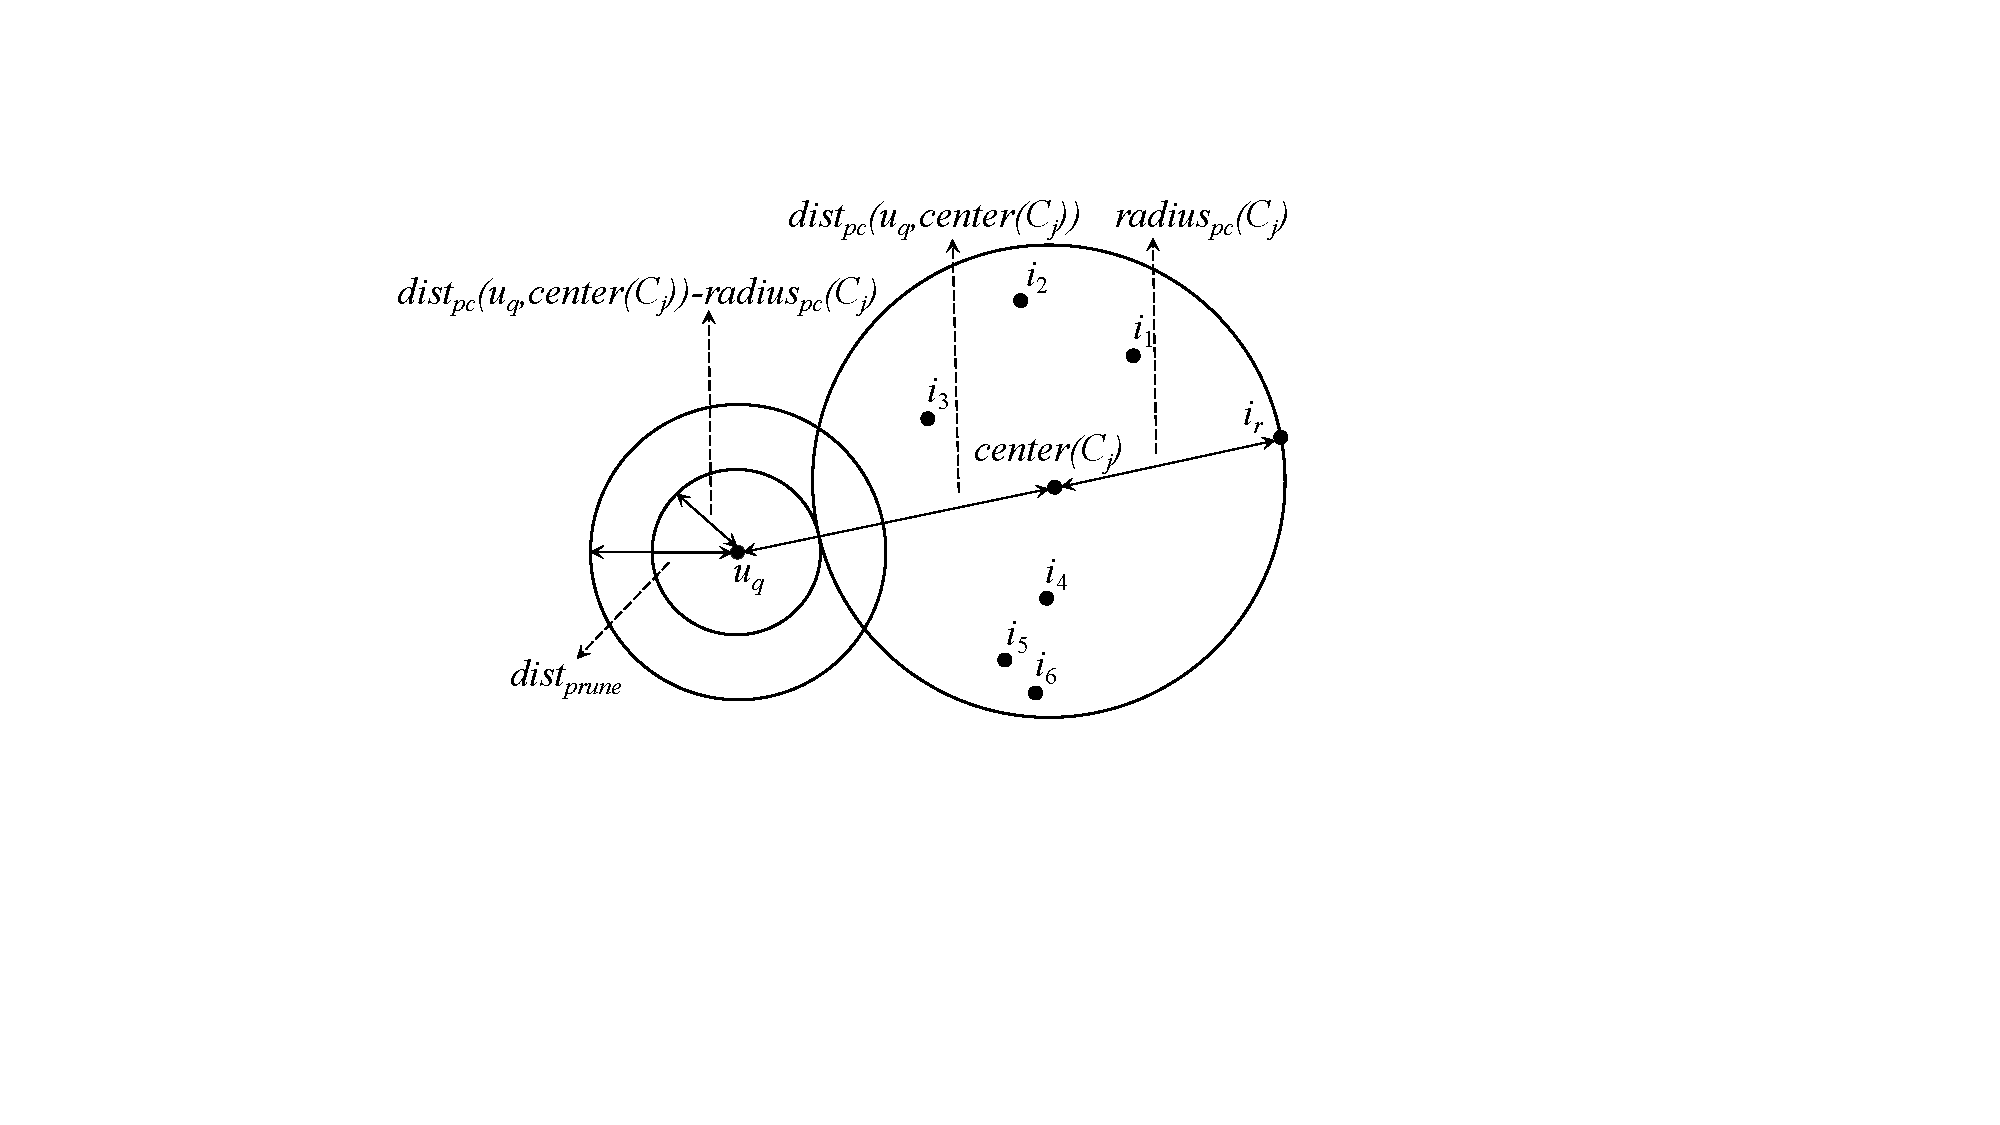
\includegraphics[width=0.41\textwidth]{Images/knn_error_11.pdf}
    \caption{Retention of remote data points that should have been pruned in the kNN search process on \dualtree.}
    \label{fig:knn_error}
\end{figure}

\begin{figure}[t]
    \centering
    \hspace*{0.15cm}    
    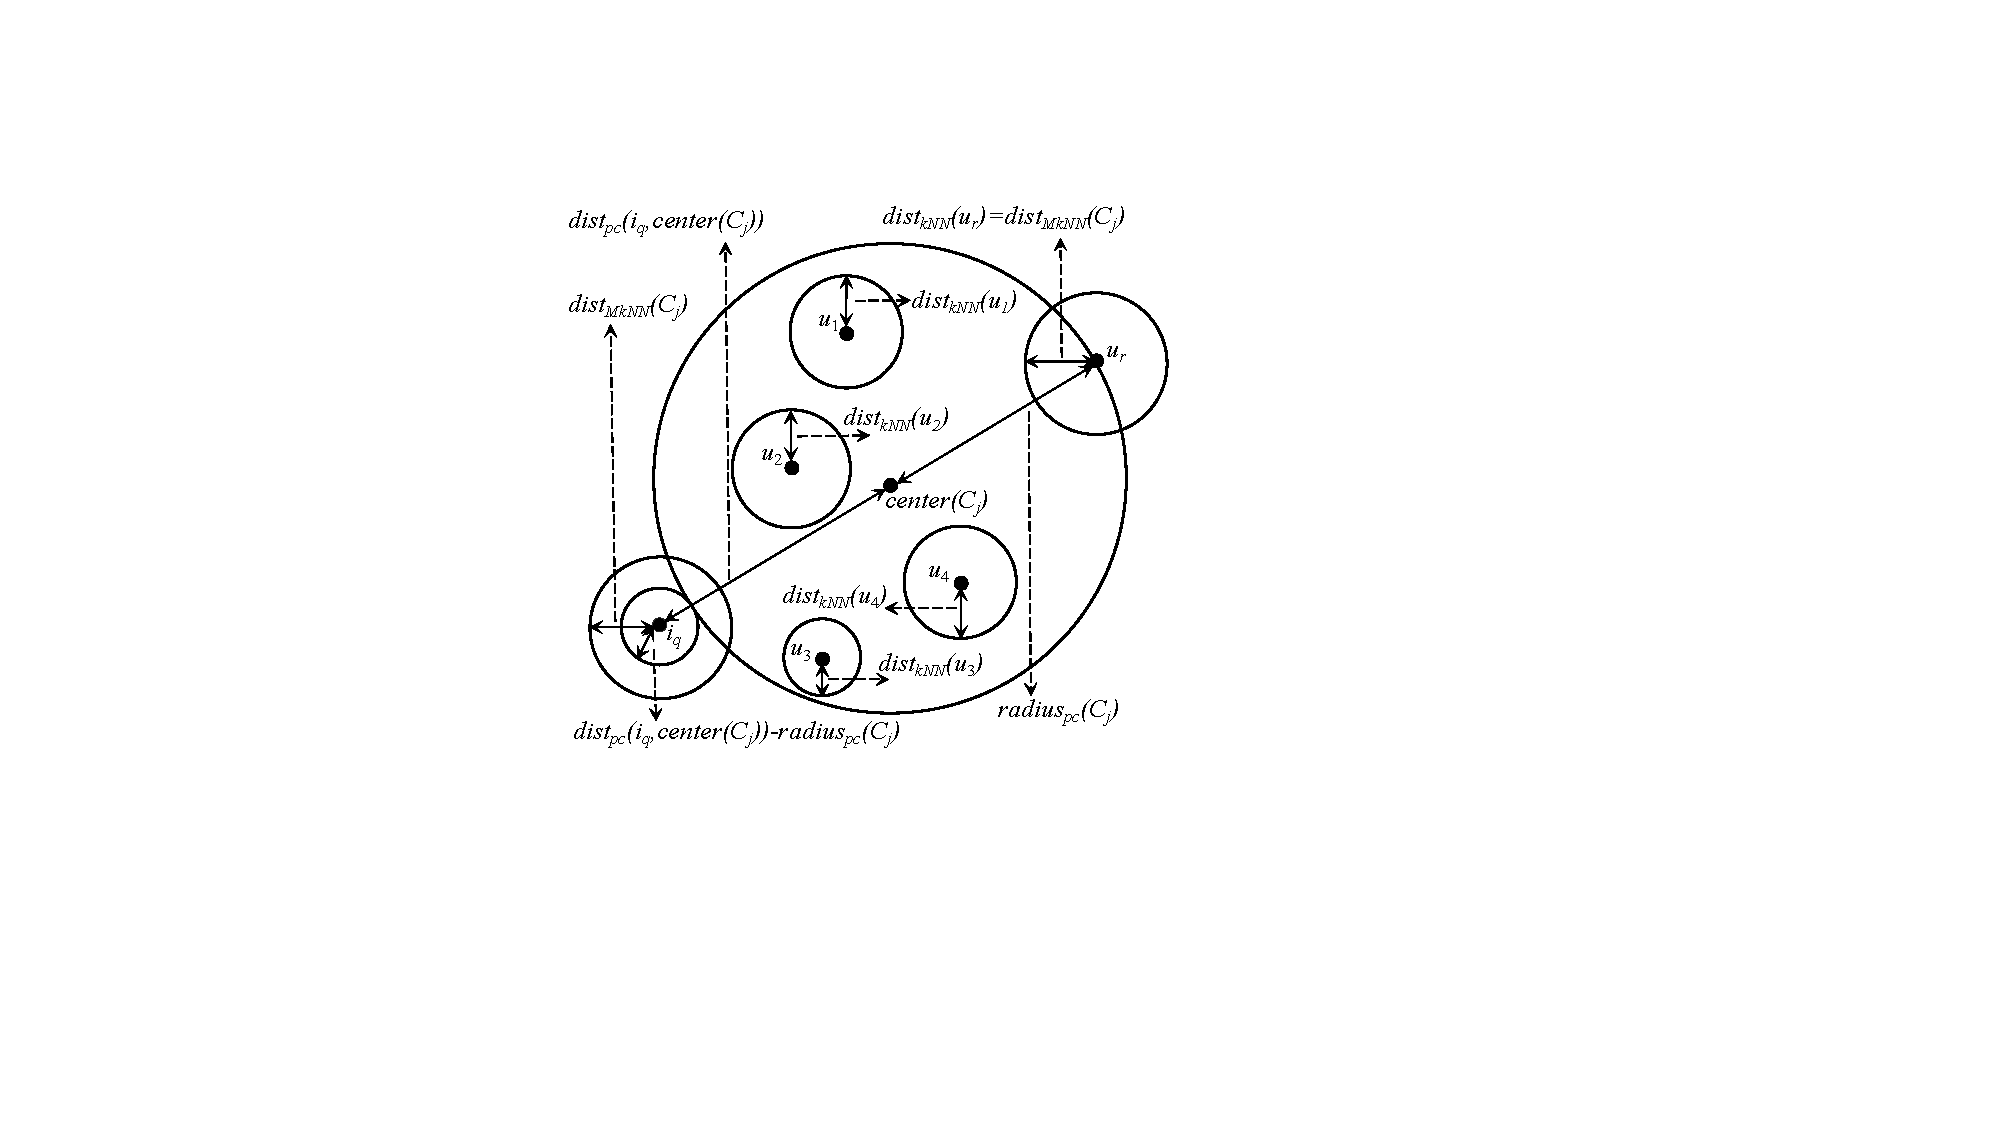
\includegraphics[width=0.4\textwidth]{Images/rknn_error_26.pdf}
    \caption{Retention of remote data points that should have been pruned in the RkNN search process on \dualtree.}
    \label{fig:rknn_error}
\end{figure}


\begin{example}[False positive error in kNN search]
In Figure \ref{fig:knn_error}, a cluster $C_j$ at a non-leaf node in the \deltatree part of \dualtree is visited during kNN search for query point $u_q$. The cluster is retained because the lower-bound test $dist_{PC}(center(C_j), u_q)-radius_{PC}(C_j)<dist_{prune}$ holds. The far-side point $i_r$ determines the large value of $radius_{PC}(C_j)$ and keeps this lower bound below $dist_{prune}$. Nevertheless, every point in $C_j$ is actually farther from $u_q$ than $dist_{prune}$, so the cluster survives only because the test is applied to the cluster as a whole rather than to its member points.  
\label{example:false positive error in kNN Search}
\end{example}

\begin{example}[False positive error in RkNN search]
In Figure \ref{fig:rknn_error}, a cluster $C_j$ at a non-leaf node in the \hdrtree part of \dualtree is visited during RkNN search for query point $i_q$. The cluster is retained because the lower-bound test $dist_{PC}(center(C_j), i_q)-radius_{PC}(C_j)<\dmknn(C_j)$ holds. The far-side point $u_r$ determines the large value of $radius_{PC}(C_j)$ and keeps this lower bound below $\dmknn(C_j)$. Nevertheless, for every data point $u\in C_j$, the distance from $i_q$ to $u$ still exceeds $\dmknn(C_j)$, so no point in the cluster should survive once point-to-point checking is performed.  
\label{example:false positive error in RkNN Search}
\end{example}

The false-positive errors in Example \ref{example:false positive error in kNN Search} and Example \ref{example:false positive error in RkNN Search} arise because the points $i_r$ and $u_r$, which respectively determine the large cluster radii, are positioned on the far side relative to the query points $u_q$ and $i_q$. This spatial misalignment keeps the cluster-level lower bound loose, so the test remains correct while still leaving member points that can be pruned once point-to-point distances are examined.

In short, non-leaf pruning on \dualtree is effective but intentionally conservative. It narrows the search space substantially, yet it can still leave a nontrivial number of point-level false positives at the leaf nodes. This motivates an additional pruning step at the leaf level, applicable to both the \hdrtree and \deltatree parts of \dualtree, based on low-dimensional point-to-point distance computation. The remaining question is then no longer whether such pruning is correct, but how many dimensions should be used so that the extra pruning power outweighs the cost of the added distance computations.

\subsection{Point-level pruning}

Because non-leaf pruning on \dualtree is cluster-based and intentionally conservative, some distant false positives inevitably reach the leaf nodes and create avoidable overhead for the final full-dimensional verification. We reduce this overhead by introducing an intermediate point-wise pruning stage at the leaf level. This stage performs a low-dimensional distance check before the expensive full-dimensional evaluation.

\noindent\textbf{Point-wise pruning step.}
Let $q$ denote the search-originating point and $v$ denote a point visited at a leaf node. Their roles and the pruning threshold $b_p$ are specified as follows:
\begin{itemize}
\setlength{\itemsep}{0pt}
\setlength{\parsep}{0pt}
\setlength{\topsep}{0.2ex}
\setlength{\leftmargin}{1.4em}
\item \textbf{kNN search on the \deltatree:} $q\in U$ is a query, $v\in I$ is a reference point, and $b_p$ is the current $k$-th best distance.
\item \textbf{RkNN search on the \hdrtree:} $q\in I$ is a reference, $v\in U$ is a query point, and $b_p$ is the stored kNN distance of $v$, i.e., $\dknn(v,I)$.
\end{itemize}
Let $dist_{PC}$ be the distance of two points in the selected principal-component space. If $dist_{PC}(q,v) \ge b_p$, then $v$ can be safely pruned because $dist(q,v)\ge dist_{PC}(q,v)\ge b_p$, according to Lemma \ref{lm:pca_decrease_dist}. This step therefore provides a unified leaf-level filter for both kNN search on the \deltatree\ and RkNN search on the \hdrtree.

The effectiveness of this stage depends on one critical question: what is the optimal projection dimensionality $d$ for this check? The choice involves a fundamental trade-off: a higher $d$ offers stronger pruning power but also increases the cost of the check itself. To address this trade-off, we develop a cost-aware mathematical model that relates the pruning dimensionality to the expected computational overhead and thereby identifies the theoretically optimal value of $d$.

The goal of selecting an optimal number of pruning dimensions is to minimize the expected computational cost for a randomly visited data point on a leaf node of \dualtree during the search process for a randomly selected search-originating data point. We first formulate a cost model that expresses the expected cost as a function of the pruning dimensionality, $d$. We then derive the optimal pruning dimensionality by applying optimization methods to this model.

While leaf-node processing involves minor operations like bound comparisons and inserting the visited point into the RkNN list or the list containing the candidate kNN members of the query origin, their computational cost in high-dimensional settings is overwhelmingly dominated by distance calculations. Our cost model therefore focuses exclusively on this dominant factor. We model the cost by defining a unit cost $c$ as the expense of a single-dimension squared difference and addition within a Euclidean distance computation. Consequently, a $d$-dimensional distance check incurs a cost of approximately $dc$.

Let $d$ be the pruning dimensionality and $D$ be the full dimensionality. For any visited point at a leaf node, there are three possible outcomes based on our pruning rule:

\noindent \textit{Situation 1}: True Candidate: The point should be accepted. It passes the $d$-dim check and requires a full $D$-dim verification. The total cost is $(d+D)c$. This occurs with probability $P_a$.

\noindent \textit{Situation 2}: False Positive (Pruned): The point is not a neighbor and is successfully pruned by the $d$-dim check. The cost is only $dc$. This occurs with probability $P_p(d)$.

\noindent \textit{Situation 3}: False Positive (Not Pruned): The point is not a real kNN candidate or a RkNN member of the query origin but survives the $d$-dim check, requiring a full $D$-dim verification to be discarded. The total cost is $(d+D)c$. This occurs with probability $1 - P_a - P_p(d)$.


By summing the costs of these mutually exclusive outcomes and simplifying the full expectation, we obtain
\begin{equation}
E_{cost(q,v)}(d)=(D-D\cdot P_p(d)+d)c .
\end{equation}

To minimize this cost, our central challenge reduces to accurately modeling the pruning probability function, $P_p(d)$. To develop a tractable model for this function, we assume that the data distribution remains relatively stable throughout the update process and formalize the statistical properties of the process below. Before detailing these properties, we define the minimal bounding hyperrectangles, $\mathcal{O}_U$ and $\mathcal{O}_I$, that respectively enclose all points of $U$ and $I$ during the update process:
\begin{align}
    \mathcal{O}_U &= \{P \mid \forall j\in[1,D], u[j]_{\min} \le P[j] \le u[j]_{\max}\} \nonumber \\
    \mathcal{O}_I &= \{P \mid \forall j\in[1,D], i[j]_{\min} \le P[j] \le i[j]_{\max}\} \nonumber
\end{align}
Here, $u[j]_{\min}$, $u[j]_{\max}$ and $i[j]_{\min}$, $i[j]_{\max}$ are respectively the minimum and maximum coordinates observed in the set $U$ and $I$ during the update process. For subsequent discussions, we use $\mathcal{O}$ as a collective term for both $\mathcal{O}_U$ and $\mathcal{O}_I$ when the context is clear.

We assume that, during the update period, the following objects exist:

\begin{itemize}
\setlength{\itemsep}{0pt}
\setlength{\parsep}{0pt}
\setlength{\topsep}{0.2ex}
\setlength{\leftmargin}{1.4em}
\item \textbf{Partition:} $\{\mathcal{O}^i\}_{i=1}^{M}$, where $\mathcal{O}=\bigcup_{i=1}^{M}\mathcal{O}^i$.
\item \textbf{Region probability:} $P_i$ for $1\leq i\leq M$.
\item \textbf{Bound count:} integer $B_i$ for $1\leq i\leq M$.
\item \textbf{Bound-kernel probability:} $\pi_{ij}$ for $1\leq i\leq M$ and $1\leq j\leq B_i$, denoting the probability of the $j$-th representative pruning bound in $\mathcal{O}^i$.
\item \textbf{Local density:} $f_{ij}$ for $1\leq i\leq M$ and $1\leq j\leq B_i$, denoting the density associated with the $j$-th representative pruning bound in $\mathcal{O}^i$.
\end{itemize}

These objects ensure that the following properties hold throughout the update process. Note that the notation $\mathcal{O}$ is used in this paper as a collective reference to both $\mathcal{O}_U$ and $\mathcal{O}_I$, which does not imply that $\mathcal{O}_U = \mathcal{O}_I$. When $\mathcal{O} = \mathcal{O}_U$ and $\mathcal{O} = \mathcal{O}_I$, respectively, the aforementioned objects may differ.


\noindent \textit{Property 1}: For a randomly selected search-originating point $q$, the probability of $q$ being included in $\mathcal{O}^i$ is approximately equal to $P_i$, that is, $P(q\in \mathcal{O}^i)\approx P_i$. 

\noindent \textit{Property 2}: When $\mathcal{O}=\mathcal{O}_{U}$, for a random point $q$ with $q\in \mathcal{O}^i$, the number of distinct pruning bound values encountered during the search of $q$ is $B_i$. When $\mathcal{O}=\mathcal{O}_{I}$ and the data point $q$ requiring RkNN search belongs to $\mathcal{O}^i$, the pruning bound values encountered during the search of $q$ tend to cluster around $B_i$ distinct representative values. In this paper, we refer to these representative values, around which the pruning bound values concentrate, as \emph{bound kernels}.

\noindent \textit{Property 3}: For a random visited data point $v$ at the leaf level of \dualtree during the search process of a random data point $q$, the conditional probability that $v$ encounters the $j$-th ($1\leq j\leq B_i$) pruning bound value (bound kernel) $b_{p}(q,j)$, that is, $b_p=b_{p}(q, j)$, when $q\in \mathcal{O}^i$, is given by $P(b_p=b_{p}(q, j)|q\in \mathcal{O}^i)\approx \pi_{ij}$. 

\noindent \textit{Property 4}: Let $q_{\mathcal{O}^i}$ be an arbitrary search origin in $\mathcal{O}^i$, and let $v^{j}_{q_{\mathcal{O}^i}}$ be a random visited data point that encounters the $j$-th pruning bound (bound kernel) $b_{p}(q_{O^i},j)$ during the search of $q_{O^i}$. Treat $q_{O^i}$ as a fixed point, and define $Z_{ij}=dist^2(q_{\mathcal{O}^i},v^{j}_{q_{\mathcal{O}^i}})/b^{2}_{p}(q_{O^i},j)$. Then $Z_{ij}$ is a random variable because $v^{j}_{q_{\mathcal{O}^i}}$ is random. Its density, written as $f_{Z_{ij}}(q_{\mathcal{O}^i},x)$, shows minimal sensitivity to the specific position of $q_{\mathcal{O}^i}$ within $\mathcal{O}^i$ and is approximately equal to $f_{ij}$. Hence, $f_{Z_{ij}}(q_{\mathcal{O}^i},x)$ can also be written as $f_{Z_{ij}}(x)$. In conclusion, the following approximation can be deduced:

For compact notation, let $Z=dist^2(q,v)/b_p^2$. The approximation above can then be written as
\begin{equation}
f_{Z\mid q\in \mathcal{O}^i,\,b_p=b_p(q,j)}(x)
\approx f_{Z_{ij}}(x)
\approx f_{ij}(x).
\label{equ: local_distribution}
\end{equation}

In the approximation above, $f_{Z\mid q\in \mathcal{O}^i,\,b_p=b_p(q,j)}$ is the density of $Z$ under the condition that $q\in\mathcal{O}^i$ and the visited point encounters the $j$-th pruning bound. For convenient expression, the term \emph{local distribution} refers uniformly to $f_{Z\mid q\in \mathcal{O}^i,\,b_p=b_p(q,j)}$, $f_{Z_{ij}}$, and $f_{ij}$, which are equivalent by Property 4.  

\noindent\textbf{Rigorous pruning probability.} Based on the settings and conditions above, the function $P_p(d)$ can now be analyzed. As discussed earlier, $P_p(d)$ represents the probability that $v$ should not be included in either the RkNN list or the candidate kNN list of $q$ and can therefore be pruned through low-dimensional distance computation. This gives
\begin{flalign}
P_p(d)&=P(dist_{PC}(q,v)\geq b_p)\nonumber \\
&=P(\frac{dist^2(q,v)}{b_p^2}\geq \frac{dist^2(q,v)}{dist_{PC}^2(q,v)})  
\label{equ: ped_basic}
\end{flalign}
To formulate $P_p(d)$, we study the density $f_{dist^2(q,v)/b_p^2}$ of the random variable $dist^2(q,v)/b_p^2$ together with the relationship between $d$ and $dist^2(q,v)/dist_{PC}^2(q,v)$. For convenient expression, we use the term \emph{global distribution} to refer to the distribution of the random variable $dist^2(q,v)/b_p^2$ in the subsequent discussion.


\noindent\textbf{\textit{Distance shrinkage.}} To study the relation between $d$ and the square rate $dist^2(q,v)/dist^2_{PC}(q,v)$ between the full-dimensional distance and the low-dimensional distance computed on a subset of principal component dimensions, we revisit a basic property of PCA. The eigenvalue $e_i$ of the covariance matrix of the initial state of $U\cup I$ before the updates start, corresponding to the $i$th row vector of the PCA projection matrix $M$, is equal to the variance $\sigma^2_i$ of the data-point coordinates in the initial $U\cup I$ along the $i$th dimension $PC(i)$ of the PC space. Here, $\sigma^2_i$, defined as $\frac{\sum_{p\in U\cup I}(p_{PC(i)}-\overline{p_{PC(i)}})^2}{|U\cup I|}$, represents the degree of dispersion of the data points along that dimension. Consequently, given the pruning dimensionality $d$ and the number of full dimensions $D$, the following approximation can reasonably be made:
\begin{flalign}
    \frac{dist^2(v,q)}{dist_{PC}^2(v,q)}\approx\frac{\sum_{i=1}^{D}\sigma^2_i}{\sum_{i=1}^{d}\sigma^2_i}= \frac{\sum_{i=1}^{D}e_i}{\sum_{i=1}^{d}e_i} 
\end{flalign}

Because the row vectors in the PC matrix are sorted in descending order by their corresponding eigenvalues, the quantity $ \frac{\sum_{i=1}^{d}e_i}{\sum_{i=1}^{D}e_i}$ increases rapidly when $d$ is small and then slows as $d$ grows, yielding a curve that rises sharply at first and gradually flattens in the coordinate system whose X-axis is $d$ and whose Y-axis is $ \frac{\sum_{i=1}^{d}e_i}{\sum_{i=1}^{D}e_i}$. Therefore, a function of the form $kln(d)+b$, which exhibits a similar curve shape, can be used to approximately model the relationship between $ \frac{\sum_{i=1}^{d}e_i}{\sum_{i=1}^{D}e_i}$ and $d$. As a result, the functional model $kln(d)+b$ can also be applied to $dist_{PC}^2(q,v)/dist^2(q,v)$, which can be written in the following mathematical form:
\begin{flalign}
    \frac{dist_{PC}^2(v,q)}{dist^2(v,q)}\approx \frac{\sum_{i=1}^{d}e_i}{\sum_{i=1}^{D}e_i}\approx kln(d)+b 
\end{flalign}

Given this approximation to $dist_{PC}^2(q,v)/dist^2(q,v)$, the remaining task is to determine the two parameters $k$ and $b$. Let $\rho_1=e_1/\sum_{i=1}^{D}e_i$. We fit $k\ln(d)+b$ by matching the two endpoints, namely $\rho(1)=\rho_1$ and $\rho(D)=1$. Since $\ln(1)=0$, the parameters are
\begin{equation}
b=\rho_1,\qquad k=\frac{1-\rho_1}{\ln D}.
\end{equation}

At this stage, the parameters $k$ and $b$ have been obtained, and the relation between the pruning dimensionality and the square rate between the full-dimensional and low-dimensional distances has been derived. We next turn to the global distribution in order to connect the pruning dimensionality to the pruning probability.

\noindent\textbf{\textit{Global distribution.}} We next turn to the random variable $dist^2(q,v)/b_p^2$. The remaining task is to characterize its density $f_{dist^2(q,v)/b_p^2}$, because together with the distance-shrinkage model above it determines $P_p(d)$. According to Property 4, the global distribution can be derived from the corresponding local distributions. Under the conditions assumed above, the law of total probability and Bayes' theorem yield the following lemma.
\begin{lemma}{(Model of global distribution).}
The global distribution is a linear combination of local distributions. In mathematical form, it can be written as:
$f_Z(x)\approx \sum^{M}_{i=1}\sum^{B_i}_{j=1} P_i\pi_{ij}f_{ij}(x)$   
\end{lemma}
\label{thm:framework_F}
\begin{proof}
Because of the Law of Total Probability, the approximation below holds throughout the update process:
\begin{flalign}
f_{dist^2(q,v)/b^2_p}&=\sum^{M}_{i=1}P(q\in \mathcal{O}^i)f_{(dist^2(q,v)/b^2_p|q\in \mathcal{O}^i)} \nonumber   \\
&\approx \sum^{M}_{i=1}P_if_{(dist^2(q,v)/b^2_p|q\in \mathcal{O}^i)}  
\label{equ:F_general_domain_partiton}
\end{flalign}

Because of the Law of Total Probability and Properties 2--4, the conditional density of $Z$ in region $\mathcal{O}^i$ can be decomposed by pruning-bound kernels. Let $p_{ij}=\Pr(b_p=b_p(q,j)\mid q\in\mathcal{O}^i)$. Then
\begin{equation}
\begin{aligned}
f_{Z\mid q\in\mathcal{O}^i}(x)
&= \sum^{B_i}_{j=1} p_{ij}\,
f_{Z\mid q\in\mathcal{O}^i,\,b_p=b_p(q,j)}(x) \\
&\approx \sum^{B_i}_{j=1} \pi_{ij}f_{ij}(x).
\end{aligned}
\label{equ:F_general_pruningboundpartition}
\end{equation}
Therefore, $f_Z(x)\approx \sum^{M}_{i=1}\sum^{B_i}_{j=1} P_i\pi_{ij}f_{ij}(x)$ holds during the update process.
\end{proof}




To complete the global model, it remains to characterize $f_{ij}$ for $1\leq i\leq M$ and $1\leq j \leq B_i$. According to Property 4, $f_{dist^2(q_{\mathcal{O}^i},v^{j}_{q_{\mathcal{O}^i}})/b^{2}_{p}(q_{O^i},j)} \approx f_{ij}$ regardless of the specific position of $q_{\mathcal{O}^i}$ in $\mathcal{O}^i$. It is therefore sufficient to analyze the local distribution obtained by fixing an arbitrary query point $q_{\mathcal{O}^i}$ in $\mathcal{O}^i$ and treating $v^{j}_{q_{\mathcal{O}^i}}$ as a random visited point that encounters the $j$-th pruning bound (bound kernel) in the search of $q_{\mathcal{O}^i}$. The following lemma states the resulting approximation.


\begin{lemma}{(Local distribution.)}
The local distribution is approximately a Normal distribution, which can be written in mathematical form as $\frac{dist^2(q_{\mathcal{O}^i},v^{j}_{q_{\mathcal{O}^i}})}{b^2_{p}(q_{O^i},j)} \sim \mathcal{N}(\mu, \sigma^2)$.

\label{thm:normal_distribution_local}
\end{lemma}
The proof for lemma \ref{thm:normal_distribution_local} is presented in Appendix A.1 and A.2.

As a result, the global distribution, that is, the distribution of $Z=dist^2(q,v)/b_{p}^2$, is a mixed Normal distribution. Let
\[
\phi_m(x)=\frac{1}{\sqrt{2\pi\sigma^2_m}}\exp\left(-\frac{(x-\mu_m)^2}{2\sigma^2_m}\right)
\]
denote the density of the $m$-th Normal component. The global density can then be formulated as
\begin{equation}
f_Z(x)\approx \sum^{T}_{m=1}p_m\phi_m(x),
\end{equation}
 where $T=\sum^{M}_{i=1}B_i$, and $\mu_m$ and $\sigma^2_{m}$ are respectively the expected value and variance of the $m$-th Normal Distribution.

After formulation of the distribution model of $Z$, the parameters in the model should be further estimated to derive the concrete $f_Z(x)$. The detailed discussion is presented in Appendix A.3


At this stage, we have derived the relationship between the pruning dimensionality $d$ and the square rate $dist^2(q,v)/dist^2_{PC}(q,v)$, as well as the approximate global distribution of $Z$. Let $a(d)=1/(k\ln(d)+b)$ denote the approximate lower bound induced by the distance-shrinkage model. Since pruning occurs when $Z\geq dist^2(q,v)/dist^2_{PC}(q,v)$, the pruning-probability function can be written as:







\begin{equation}
P_p(d)=\int_{a(d)}^{+\infty} f_Z(x)\mathrm{d}x
\approx \int_{a(d)}^{+\infty}\sum^{T}_{m=1}p_m\phi_m(x)\mathrm{d}x .
\label{equ:ppd}
\end{equation}
Afterward, the optimal $d$ can be determined by finding the extremum of $E_{cost(q,v)}(d)$ to achieve minimization.

\noindent\textbf{Simplified pruning probability.}
Before deriving the extremum of $E_{cost(q,v)}(d)$, we introduce a simplified method to compute an approximation to the function $P_p(d)$ between the pruning probability and the pruning dimensionality. Although this simplified approach provides a less precise relationship than the more rigorous method discussed earlier, experimental results show that the optimal pruning dimensionality derived from it still delivers satisfactory computational efficiency.

The proportion of the total variance accounted for by the first $d$ principal component dimensions is positively related to the pruning probability, because a higher variance proportion means that more distance information is preserved. Heuristically, it is therefore reasonable to assume that the pruning probability $P_p(d)$ has a positive linear relationship with $\sum^{d}_{i=1}e_i/\sum^{D}_{i=1}e_i$, which can in turn be approximated by the functional model $kln(d)+b$. Let $k''=k'k$ and $b''=k'b+b'$. As a result, the model below can be used to approximate $P_p(d)$:
\begin{equation}
    P_p(d)\approx k''ln(d)+b''.
\label{equ:simppd} 
\end{equation}

The parameters $k''$ and $b''$ can be estimated by a sampling method. For the pruning probability at leaf nodes of the \deltatree part of \dualtree, before the update starts, $10\%$ data points at each leaf node of the \hdrtree part should be sampled, and kNN search for them using two different pruning dimensions $d_1$ and $d_2$ should be implemented on initial $I$, and the two pruning frequencies $P^1_p$ and $P^2_p$ should be recorded. Subsequently, the equation system below can be used to determine $k''$ and $b''$:
\begin{flalign}
    P^1_p=k''ln(d_1)+b'' \quad
    P^2_p=k''ln(d_2)+b''
\end{flalign}
    
For the pruning probability at leaf nodes of the \hdrtree part of \dualtree, before the updates start, $10\%$ data points at each leaf node of the \deltatree part should be sampled, and RkNN search for them using two different pruning dimensions $d_1$ and $d_2$ should be implemented on initial $U$, and the two pruning frequencies $p^1_e$ and $p^2_e$ should be recorded. Subsequently, the same equation system presented above can be used to confirm $k''$ and $b''$.

In conclusion, a simplified linear-log model, $k''ln(d)+b''$, is observed to approximate the function model of pruning probability $P_p(d)$ over the pruning dimensionality $d$. The estimation of the parameters $k''$ and $b''$ is performed before the update starts. These two parameters should be re-computed when the performance of the newly added pruning step decreases below a specific threshold after a long phase.



\noindent\textbf{Optimal pruning dimensionality.}
For the strict pruning probability function in expression \ref{equ:ppd}, let $S(d)=\sum^{T}_{m=1}p_m\phi_m(a(d))$ denote the mixed density evaluated at the lower bound $a(d)$. Differentiating $a(d)=1/(k\ln(d)+b)$ gives
\begin{equation}
\frac{\mathrm{d}E_{cost(q,v)}(d)}{\mathrm{d}d}
\approx 1-\frac{kD}{d(k\ln(d)+b)^2}S(d).
\end{equation}

Setting this derivative to zero gives
\begin{equation}
\frac{kD}{d(k\ln(d)+b)^2}S(d)=1 .
\end{equation}
This transcendental equation is solved numerically over $[1,D]$. We then evaluate $E_{cost(q,v)}(d)$ at $1$ and at the neighboring integers of the approximate roots, and choose the value of $d$ with the minimum cost. 

For the simplified pruning probability function in expression \ref{equ:simppd}, $\mathrm{d}E_{cost(q,v)}(d)/\mathrm{d}d=c(-Dk''/d+1)$. Since $k''>0$, the derivative is zero at $d=Dk''$, negative when $d<Dk''$, and positive when $d>Dk''$. Hence, the simplified model yields the approximate optimum $d^*=Dk''$.

The foregoing discussion determines the pruning dimensionality used at the leaf level of \dualtree. It reduces the verification cost caused by points that are not kNN candidates or RkNN members but survive non-leaf pruning. 

























